\chapter{La prédiction du mécanisme de récupération}

\section{Introduction}
Notre étude a pour objectif la prédiction de la meilleure stratégie de récupération en cas de pannes dans un Web Service Composite en se basant sur un ensemble d'informations concernant les Web services composé et la qualité de service.

L'approche proposé dans ce présent mémoire se base sur la notion de l'auto-apprentissage (Machine Learning), L'ensemble des données généré dans l'étude précédente cité dans le chapitre "État de l'art", vont être traité et exploité comme des données d'apprentissage, pour qu'on puisse après prédire d'une manière automatique et dynamique le mécanisme de récupération le mieux adapté.

Le présent chapitre décris d'une part les différent problématiques de l'auto-apprentissage ainsi que le type de problématique dans lequel se situe notre approche de prédiction, d'autre part on va présenter les deux étapes principaux de l'approche, le traitement et l'intégration des données en utilisant Pentaho et la prédiction des mécanismes de récupération en appliquant les algorithmes de Machine Learning via l'outil Weka. 


\section{L'auto Apprentissage -Machine Learning- }

L'apprentissage automatique -Machine Learning- est un domaine de l'intelligence artificielle qui consiste en général une manière de traitement d'un ensemble de données pour un apprentissage automatisé de la machine ou de l'ordinateur afin de pouvoir effectuer des opérations complexes.

Un algorithme de machine Learning se différencie des autres algorithmes classiques à travers la notion de l'apprentissage, car un algorithme de Machine Learning s'améliore par lui même à partir des données sans supervision d'un être humain.

Pour bien définir un problème de machine learning, il faut bien définir quatre element principaux: 

- Les données

- La tache à accomplir 

- L'algorithme d'apprentissage

- La mesure de performance


Les données : représente l'ensemble de base d'information sur lesquelles se base l'apprentissage automatique, notre approche se base sur les données générées par le système d'exécution des services Web Composite cité dans l'Etat de l'art.

La tache spécifique : Le Machine Learning a besoin de la définition d'une tâche spécifique à accomplir c'est à dire  qu'est ce qui peut répondre au problème, une tâche peut être sous forme d'une prédiction, identification, recommandation... 

L'algorithme : Après la définition de la tâche spécifique et les données nécessaires pour la traiter, On peut passer à la troisième étape qui consiste le choix d'un algorithme spécifique qui va pouvoir répondre à la tache à partir des données collectée. il existe plusieurs algorithmes de Machine Learning ( Réseau de neurones, Support vector machine, Régression linéaire ... ), le choix de l'algorithme dépend de la nature et le type de la problématique de machine Learning.

La mesure de performance : Une fois l'algorithme est déterminé, il faut choisir une mesure de performance relativement à la tache définie précédemment en s'appuyant sur des métriques précises.  

Un process de Machine Learning passe par deux phases principales, La première phase c'est la phase où l'être humain sera responsable du choix et de l'entraînement de l'algorithme d'apprentissage, pour que le traitement de la tache spécifique sera appris à partir de l'apprentissage (Training set), pour que l'algorithme dans la deuxième phase effectue la tâche lui même.

\begin{figure}[H]
\begin{center}
\includegraphics[width=1\linewidth]{images/auto apprentissage.png}
\end{center}
\caption{Processus du Machine Learning}
\label{fig:6}
\end{figure}

\subsection{Choix de l'algorithme de Machine Learning}

Le choix de l'algorithme auquel  on va avoir besoin de faire appel pour le traitement de la problématique nécessite tout d'abord  la distinction des différents types de problèmes de Machine Learning et les familles d'algorithmes associés avec leurs spécificités.

La première distinction à faire dans les problèmes de Machine Learning, c'est la détermination des problèmes supervisés (supervised learning) et des problèmes non supervisés (unsupervised learning), la seconde consiste la distinction entre un problème de Régression et un problème de Classification.

\subsubsection{Apprentissage supervisé vs non-supervisé}


- L'apprentissage supervisé : exploite exclusivement l'ensemble des données dites annotées de leur sorties pour pouvoir construire un modèle, c'est à dire que chaque donnée est associée à une classe cible ou une catégorie et l'objectif c'est que l'algorithme soit capable de prédire cette classe sur des nouvelles données qui ne sont pas annotées a partir du modèle qui a construit précédemment.

Représentation Mathématique : 
    
    On reçoit en entré des données d'exemple annotées:
    (x1,y1),(x2,y2),(x3,y3), ... et on veut prédire la sortie sur des nouvelles données :  x* --> y* 
    

- L'apprentissage non-supervisé : est beaucoup plus complexe puisque les données d'entrées ne sont pas annotées. l'algorithme d'entraînement va devoir dans ce cas  trouver  les similarités et distinctions au sein de ces données, et à organiser et regrouper ensemble celles qui partagent des caractéristiques communes.

Représentation Mathématique : 
    
    On reçoit en entré uniquement des données brutes de variables aléatoire : x1,x2,x3,... et on veut avoir la relation avec des variables latentes structurelles :  xi --> yi 
    
En plus de ces deux principaux familles d'algorithme (Supervisé/non-Supervisé) il existe d'autre types d'apprentissage, l'apprentissage semi-supervisé qui prend en entré un mélange de données annotées et non annotées et l'apprentissage par renforcement son but est d'apprendre a partir des expériences, en gros l'algorithme de base sur un cycle d'expériences et de récompenses et il s'auto améliore à chaque itération.

\subsubsection{Classification vs Régression }

\begin{figure}[H]
\begin{center}
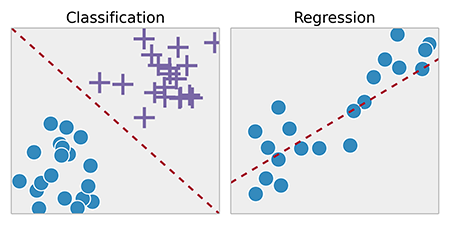
\includegraphics[width=1\linewidth]{images/ClassReg.png}
\end{center}
\caption{Différence entre Classification et Régression}
\label{fig:6}
\end{figure}

- Classification : Chaque observation ou donnée  est associée à une et une seule modalité (appelée classe/catégorie), La classification c'est le type de problème dans lequel la sortie attendu de l'algorithme est discrète c'est à dire elle est sous forme d'une catégorie ou classe.
    
- Régression : La variable de sortie de l'algorithme est quantitatif, c'est à dire elle  prend des valeurs dans un sous-domaine de l’ensemble des nombres réels. exemple: La prédiction de la rentabilité d'une compagne marketing. 


Notre problématique concerne la prédiction de la stratégie de récupération d'un service Web composite, c'est à dire prédire quelle catégorie ou classe de récupération va être mise en oeuvre, ainsi que nos données d'apprentissage sont des données qui sont générées par  un exécuteur des services Web composites vu dans l'étude précédente (Chapitre :État de l'art) et  qui permet de prendre la décision de choix de Mécanisme de récupération ce qui nous permet d'avoir un ensemble des données annotées. 
D'après cet analyse on peut situer notre problème de machine Learning dans la famille des problèmes Supervisés de Classification.

\subsubsection{Les algorithmes de Classification et Supervision}



\section{Construction du modèle de prédiction }

\subsection{Weka}
\subsection{Scikit Learn Python }

\subsection{Mesure de performance}




